%%%%%%%%%%%%%%%%%%%%%%%%%%%%%%%%%%%%%%%%%
% Stylish Article
% LaTeX Template
% Version 2.0 (13/4/14)
%
% This template has been downloaded from:
% http://www.LaTeXTemplates.com
%
% Original author:
% Mathias Legrand (legrand.mathias@gmail.com)
%
% License:
% CC BY-NC-SA 3.0 (http://creativecommons.org/licenses/by-nc-sa/3.0/)
%
%%%%%%%%%%%%%%%%%%%%%%%%%%%%%%%%%%%%%%%%%

%----------------------------------------------------------------------------------------
%	PACKAGES AND OTHER DOCUMENT CONFIGURATIONS
%----------------------------------------------------------------------------------------

\documentclass[fleqn,10pt]{SelfArx} % Document font size and equations flushed left

\usepackage{lipsum} % Required to insert dummy text. To be removed otherwise
\usepackage{graphicx}
\usepackage{subfig}
\usepackage[justification=centering]{caption}

\newcommand{\ChapterCite}[1]{\textsc{Kapitel~\ref{#1}}}

%----------------------------------------------------------------------------------------
%	COLUMNS
%----------------------------------------------------------------------------------------

\setlength{\columnsep}{0.55cm} % Distance between the two columns of text
\setlength{\fboxrule}{0.75pt} % Width of the border around the abstract

%----------------------------------------------------------------------------------------
%	COLORS
%----------------------------------------------------------------------------------------

\definecolor{color1}{RGB}{0,0,90} % Color of the article title and sections
\definecolor{color2}{RGB}{0,20,20} % Color of the boxes behind the abstract and headings

%----------------------------------------------------------------------------------------
%	HYPERLINKS
%----------------------------------------------------------------------------------------

\usepackage{hyperref} % Required for hyperlinks
\hypersetup{hidelinks,colorlinks,breaklinks=true,urlcolor=color2,citecolor=color1,linkcolor=color1,bookmarksopen=false,pdftitle={Title},pdfauthor={Author}}

%----------------------------------------------------------------------------------------
%	ARTICLE INFORMATION
%----------------------------------------------------------------------------------------

\JournalInfo{Journal, Vol. XXI, No. 1, 1-5, 2013} % Journal information
\Archive{Additional note} % Additional notes (e.g. copyright, DOI, review/research article)

\PaperTitle{Coalition skill games with incomplete information and over-abundance of tasks} % Article title

\Authors{Mihail Bogojeski, Tobias Pockrandt, Mitja Phillip Richter, Björn Fischer} % Authors


\Keywords{coalition games --- skills --- incomplete information --- matching problem} % Keywords - if you don't want any simply remove all the text between the curly brackets
\newcommand{\keywordname}{Keywords} % Defines the keywords heading name

%----------------------------------------------------------------------------------------
%	ABSTRACT
%----------------------------------------------------------------------------------------

\Abstract{In diesem Paper stellen wir einen Lösungsansatz für das Matching von Agenten mit gewissen Fertigkeiten auf Aufgaben, welche besagte Fertigkeiten benötigen. Das Ziel ist es bei Fehlen von vollständiger Information eine Maximierung der sozialen Wohlfahrt zu erreichen. Hierzu werden verschiedene Methoden und Konzepte aus Bereichen wie der Spieltheorie angewandt. Der vorgestellte Lösungsansatz wird zirka 80\% der theoretisch möglichen optimalen Lösung erreichen und wir liefern eine Reihe von Maßnahmen die eine Verbesserung dieses Wertes ermöglichen sollten, beziehungsweise die Rechenzeit bei minimalem Verlust verbessern.}

%----------------------------------------------------------------------------------------

\begin{document}

\flushbottom % Makes all text pages the same height

\maketitle % Print the title and abstract box

\tableofcontents % Print the contents section

\thispagestyle{empty} % Removes page numbering from the first page

%----------------------------------------------------------------------------------------
%	ARTICLE CONTENTS
%----------------------------------------------------------------------------------------

\section*{Introduction} % The \section*{} command stops section numbering
\label{sec:introduction}

\addcontentsline{toc}{section}{Introduction} % Adds this section to the table of contents

Dieses Paper stellt einen Abschlussbericht für den Kurs \textit{Agententechnologien in der Forschung} dar und repräsentiert die im Semester erarbeiten Resultate. Das Zusammenführen von Agenten und Aufgaben im Rahmen eines Allokationsspiels ist ein äußerst komplexes Problem. Aus diesem Grund werden einige Einschränkungen vorgenommen. Es existiert ein Pool aus Fertigkeiten und zugehörigen Intensitäten. Aus diesem Pool werden die Aufgaben und die Fertigkeiten der Agenten entnommen. Zwischen der Menge von Agenten und der, der Aufgaben soll eine möglichst effiziente Zusammenführung gefunden werden. Effizienz definiert hierbei den Grad in dem die soziale Wohlfahrt maximiert wurde. Um einen erhöhten Bezug zu Realität zu erreichen besitzen die Agenten nur ein beschränktes Wissen über ihre Umgebung. Dies führt zusätzlich dazu das die beste Lösung nicht durch einfaches propagieren aller Permutationen ermittelbar ist. \\
Für die beschriebene Spezifikation des Problems wird in diesem Paper eine Lösung vorgestellt. Hierfür wird zunächst auf die genauen Rahmenbedingungen des Versuchs eingegangen (\ChapterCite{sec:Umgebung}). Im Anschluss erfolgt eine genauere Betrachtung des angewandten Algorithmus (\ChapterCite{sec:Algorithmus}) sowie der genutzten Methoden und Konzepte (\ChapterCite{sec:Methoden}). Um die Qualität der präsentierten Lösung zu bewerten wurde eine Evaluation durchgeführt (\ChapterCite{sec:Evaluation}). Den Abschluss bilden ein Ausblick über mögliche Verbesserungen (\ChapterCite{sec:Future}), sowie eine Zusammenfassung (\ChapterCite{sec:Conclusion}). 

%------------------------------------------------

\section{Versuchsumgebung und Beschreibung}
\label{sec:Umgebung}

Um eine spannende Umgebung zu erschaffen, bezieht sich der gewählte Algorithmus nicht einfach auf Agenten und Aufgaben beziehungsweise Auftragsnehmer und Firma. Ein attraktiveres und intuitives Szenario meinen wir mit Abenteurern (Agenten) und Abenteuern (Aufgaben) gefunden zu haben. Die Abenteurer werden in einer Kaschemme angeheuert, um gewisse Abenteuer gegen die Zahlung einer bestimmten Menge Gold zu erfüllen. Im folgenden wird daher auch von Abenteurern und Abenteuern gesprochen. Die Abenteurer besitzen einen von drei möglichen Skills (Fertigkeiten). Der Pool aus Skills besteht aus \textit{Kämpfen}, \textit{Verhandeln} und \textit{Schleichen}. Jeder Fertigkeit eines Agenten ist ein Power-Wert (Intensität) zugeordnet, die beschreibt wie gut er diese beherrscht. Die Abenteuer benötigen von jedem Skill einen gewissen Wert um erfüllt zu werden. Eine Abenteuer kann nicht abgeschlossen werden, solange nicht alle Anforderungen komplett erfüllt worden sind.\\

Aufgrund des Überangebots von Aufgaben existieren mehr Abenteuer als Abenteurer, beziehungsweise benötigen die Abenteuer mehr Power um geschlossen zu werden als die Agenten in ihrer Summe verfügen. Sowohl die Abenteurer als auch die Abenteuer werden in einem gewissen Rahmen zufällig generiert. Für erstere wird ungefähr die Hälfte der Gesamtpower aller Abenteuer auf die Abenteurer verteilt. Die Abenteuer unterscheiden sich in ihrer Größe (klein, mittel, groß), wobei viele kleine und wenig große Abenteuer existieren. Der Erlös einer Abenteuer im Vergleich zu ihrer Größe ist allerdings nicht linear, sondern exponentiell. Dies entspricht auch der Realitätsnähe des Versuchs, da Großprojekte in der Regel einen größeren Gewinn ausstoßen als kleinere.\\
Wie im Titel der Arbeit erwähnt, stehen in diesem Szenario nur unvollständigen Informationen zur Verfügung. Speziell bedeutet dies, dass zwar jeder Abenteurer alle Abenteuer kennt, inklusive deren Bedarf und Erlös, allerdings keine konkreten Informationen darüber besitzt, wie viele andere Agenten im Spiel sind und insbesondere nicht, welche Skills und wie viel Power sie besitzen.\\ 
In der Planungsphase des Versuchsaufbaus wurde diskutiert, mit wie vielen Skill-Arten ein Abenteurer ausgestattet werden soll: Ein Skill pro Abenteurer oder zwei bis drei. Für den Besitz von zwei bis drei Skills sprachen eine interessantere Verhandlungsphase zwischen den Abenteurern. Dagegen standen der stark erhöhte Aufwand, sowie die Realitätsnähe, da eine Firma zumeist auf eine Aufgabe spezialisiert ist. Weiterhin bestand die unbewiesene Annahme, dass sich ein Abenteurer mit mehreren Skills auch als mehrere Abenteurer mit heweils einem Skill darstellen lässt. So führte auch nicht zuletzt die Tatsache, dass hier lediglich ein relativ ausgereifter Lösungsansatz vorgestellt werden soll, zu der Entscheidung Abenteurer mit jeweils einem Skill zu verwenden. \\

Weiterhin besitzen die Agenten für jedes Abenteuer gewisse Grundkosten die anfallen und mit dem Gewinn abgedeckt werden müssen. In unserem Beispiel ist das die Beschaffung von Tränken und die Instandhaltung von Waffen und Ausrüstung. In der Realität könnte sich dies mit Fahrtkosten oder Wartung von Maschinen vergleichen lassen. Ein weiteres Ziel welches damit verfolgt wird, ist eine Erhöhung der Individualität der einzelnen Agenten. Die Abenteurer besitzen alle das gleiche Grundverhalten, sodass sich ihre Handlungen nur durch ihre eigene Power und die Grundkosten unterscheidet. Ergo gibt es hier keine risikoscheuen oder risikoaversen Agenten. Für alle Agenten existiert ein Zeitlimit (Deadline) welches bekannt ist, nach welchem keine Bewerbungen auf Abenteuer mehr möglich sind. Somit werden die Abenteurer bei fortgeschrittener Zeit auch in weniger profitablere Alternativen wechseln um noch Gewinne zu realisieren.\\
Initiale Variationen sind in diesem Szenario: Die Anzahl an Abenteurern und die der Abenteuer. Die Einhaltung der Rahmenbedingungen erfolgen anschließend automatisch. Eine genaue Beschreibung des Ablaufes des Algorithmus erfolgt im nächsten Kapitel.\\


%------------------------------------------------

\section{Algorithmusbeschreibung}
\label{sec:Algorithmus}
Zunächst erfolgt eine grobe Zusammenfassung des Algorithmus, wobei die einzelnen Bestandteile in den folgenden Unterkapiteln ausführlicher beleuchtet werden. Zu Beginn berechnen die Agenten für jedes Abenteuer ihren Nutzen. Anschließend dürfen sie sich auf bis zu vier Abenteuer bewerben. Anhand dieser Bewerbungen werden Koalitionen gebildet und die Beste anhand des Banzhaf Power Index ausgewählt. Potentieller Überschuss in den Koalitionen wird entfernt und möglichst sinnvoll an die Agenten zurückgezahlt. Erst dadurch wird ein Erreichen des maximal möglichen Erlöses möglich. Die Information über den zu erwartenden Gewinn wird an die Agenten weitergegeben, welche sich auf dieser Grundlage auf Abenteuer beziehungsweise Koalitionen festlegen. Letztlich werden die geschlossenen Abenteuer zusammen mit der eingesetzten Power aus dem Spiel entfernt und die entsprechenden Belohnungen werden an die Agenten ausgezahlt. Sofern theoretisch noch ein Abenteuer geschlossen werden kann und die Zeit noch nicht abgelaufen ist beginnt der Algorithmus in einer neuen Iteration.

\paragraph{Bewerbungsphase:}
Jeder Agent berechnet seinen Nutzen für jedes Abenteuer und bewirbt sich für maximal vier Abenteuer, die den höchsten Nutzen für ihn haben. Die Agenten bewerben sich mit ihrer gesamten verfügbaren Power. Sollte die von dem Abenteuer benötigte Power überschritten werden, bewirbt sich der Agent mit der exakt benötigten Power. Die Bewerbungen aller Agenten werden gesammelt und als Grundlage für die Koalitionsermittlung verwendet. 

\paragraph{Koalitionsermittlung:}
Für jedes Abenteuer, werden zunächst alle möglichen Koalitionen aus den Agenten, die sich für dieses Abenteuer beworben haben, gebildet. Danach werden alle Koalitionen die keine gewinnenden Koalitionen sind (die Koalitionen, die die Anforderungen des Abenteuers nicht erfüllen), eliminiert. Falls es keine Gewinnerkoalition gibt, wird die große Koalition als die vorläufige Koalition, die der Erfüllung der Anforderungen am Nächsten ist, gespeichert. Schließlich wird in der Gewinnerkoalitionen die Banzhaf Power für jeden Agent in diesem Abenteuer berechnet. In dieser Phase werden auch die Veto-Spieler in jedem Abenteuer ermittelt und ihre jeweilige Banzhaf Power mit einem bestimmten Faktor multipliziert (in unser Implementierung verdoppelt), um die Macht der Veto-Spieler im Vergleich zu den anderen Spieler zu verdeutlichen. 

\paragraph{Beste Koalition:}
Die beste Koalition eines Abenteuers wird mit einer leicht modifizierten Version des verteilten Algorithmus ermittelt. Zuerst werden die Koalitionen eliminiert, die einen nicht minimalen Überschuss an investierter Power haben. Unter Überschuss wird hier die Differenz zwischen der investierten Power der Koalition und der benötigten Power des Abenteuers für jeden Skill verstanden. Eine Koalition die einen hohen Überschuss hat ist nicht effizient, da die überflüssige Power potentiell bei anderen Abenteuern eingesetzt werden könnte. So werden auch Dummy-Spieler aus der potentiell besten Koalition entfernt, da es immer eine Koalition ohne Dummy-Spieler und mit kleinerem Überschuss gibt. Der verteilte Algorithmus wird dann auf die Koalitionen mit minimalem Überschuss angewandt, wo die beste Koalition nach elitärer Gewinnmaximierung ausgewählt wird. Genauer gesagt, die beste Koalition ist die Koalition, für die irgendein Agent die größte Gewinnschätzung hat.

\paragraph{Überschusstilgung:} 
In dieser Phase wird die überflüssige Power aus der besten Koalition entfernt und an den jeweiligen Agenten zurückgegeben. Da Power ein ganzzahliger Wert ist, kann die überschüssige Power meistens nicht gleichmäßig auf alle beteiligten Agenten aufgeteilt werden. In unserer Implementierung wird die Aufteilung des Überschusses durch eine iterierte randomisierte Prozedur realisiert. Für jeden Skill bei dem es einen Überschuss gibt, wird in jeder Iteration eine Power-Einheit einem Agenten zurückgegeben. Jeder Agent, der Power von einem Skilltyp investiert hat, kann mit einer gewissen Wahrscheinlichkeit eine Power-Einheit des Überschusses in diesem Skilltyp zurückbekommen. Die Wahrscheinlichkeit dafür ist gleich dem Anteil der investierten Power des Agenten, aus der gesamten investierten Power aller Agenten. Das heißt, dass Agenten die mehr Power aus einen Skilltyp investiert haben, mit einer höheren Wahrscheinlichkeit eine Power-Einheit aus dem Überschuss zurückbekommen. Diese Prozedur wird so oft wiederholt, bis den ganzen Überschuss aus der besten Koalition entfernt wird.
)
\paragraph{Gewinnverteilung:}
Der Gewinn wird abhängig von der Banzhaf Power der Agenten aufgeteilt. Jeder Agent in der beste Koalition bekommt den Anteil am Gesamtgewinn, der dem Anteil seiner Banzhaf Power an der aufsummierten Banzhaf Power aller Agenten entspricht. Aufgrund der Verwendung des Banzhaf Power Index ist diese Verteilung fair bezüglich der Macht der Agenten und zusätzlich auch pareto-effizient, da der gesamte Gewinn verteilt wird.

\paragraph{Festlegung auf Abenteuer/Koalition:}
Da sich die Agenten auf maximal vier Abenteuer mit ihrer gesamten Power bewerben können, muss sich danach jeder Agent auf nur ein Abenteuer festlegen. Die Entscheidung erfolgt in zwei Phasen: In der ersten Phase, wählt jeder Agent das Abenteuer aus, für welches seine Gewinnschätzung am höchsten ist. Für die zweite Phase werden diese Entscheidungen den Agenten bekannt gegeben, die sich ebenfalls für die jeweiligen Abenteuer beworben haben. Jetzt haben die Agenten die Möglichkeit ihre Entscheidung zu ändern. Diesmal entscheiden die Agenten nicht anhand ihrer Gewinnschätzung, sondern anhand ihrer Nutzenfunktion, die die Entscheidungen der anderen Agenten aus der ersten Phase miteinbezieht. Die Agenten wählen das Abenteuer mit dem größten Nutzen. Diese Entscheidung ist für die aktuelle Runde endgültig.

\paragraph{Schliessung erfüllter Abenteuer:}
Nachdem sich jeder Agent für ein Abenteuer entschieden hat, werden die Abenteuer, für welche die Gewinnerkoalition vollständig ist, dass heißt jeder Agent in der Koalition hat sich auf dieses Abenteuer festgelegt, geschlossen. Falls ein Abenteuer geschlossen wird, wird der Gewinn an die Agenten ausgezahlt, die eingesetzte Power der Agenten abgezogen und das geschlossene Abenteuer entfernt. Ab der nächste Runde kann sich kein Agent mehr für das geschlossene Abenteuer bewerben.


\section{Methoden und Konzepte}
\label{sec:Methoden}
Nun erfolgt eine Zusammenfassung der benutzten Methoden und Konzepte, welche unter anderem aus der Spieltheorie kommen. Hier werden auch getroffene Designentscheidung erläutert und Hinweise auf Veränderungen für \ChapterCite{sec:Future} gegeben.

\paragraph{Gewinnschätzung:}
Die Gewinnschätzung des Agenten für einen Abenteuer ist eine wichtige Funktion, die in vielen Teilen der Implementierung benutzt wird.
Für ein bestimmtes Abenteuer wird die Gewinnschätzung wie folgt berechnet: Falls der Agent kein Mitglied der aktuellen Gewinnerkoalition des Abenteuers ist, schätzt er, dass er seinen fairen Anteil des Gewinns bekommt. Dass heißt er erwartet den Anteil des Gewinns, der dem Anteil seiner investierte Power an der gesamten benötigten Power des Abenteuers entspricht. Falls der Agent Teil der vorläufigen großen Koalition ist, die nicht alle Anforderungen des Abenteuers erfüllen kann, schätzt der Agent ebenfalls, dass er der den Anteil des Gewinns bekommt, der dem Anteil seiner investierten Power an der gesamten Power der Koalition entspricht. Wenn der Agent ein Mitglied der aktuellen Gewinnerkolaition ist, kennt er seine Banzhaf Power für dieses Abenteuer und schätzt seinen Anteil am gesamten Gewinn anhand seines Anteils seiner Banzhaf Power an der aufsummierten Banzhaf Power aller Agenten in dieser Koalition.

\paragraph{Nutzenfunktion:}
Die Nutzenfunktion ist das wichtigste Mittel, um das verhalten der Agenten zu steuern. Die Basis des Nutzen eines Agenten in einem bestimmten Abenteuer wird aus der Gewinnschätzung minus der Kosten für das Abenteuer gebildet. Dann wird dieser Wert abhängig von den Eigenschaften des Abenteuers angepasst und daraus der endgültige Nutzen errechnet. Es werden vier Eigenschaften eines Abenteuers und die zugehörige beste Koalition unterschieden:
\begin{itemize}
  \item[E1] Die Anzahl der bisherigen Fehlversuche in diesem Abenteuer. Eine frühere Bewerbung zählt als Fehlversuch, wenn der Agent mit dieser Bewerbung kein Mitglied der Gewinnerkoalition werden konnte.
  \item[E2] Noch benötigte Power. Es wird der Anteil der fehlenden Power, die die vorläufige große Koalition zur Schließung des Abenteuers an der gesamten benötigten Power für das Abenteuer berechnet. Diese Eigenschaft spielt nur dann eine Rolle, wenn keine Koalition gebildet werden konnte, die das Abenteuer geschlossen hätte.
  \item[E3] Anzahl der Skills, bei denen die vorläufige große Koalitionen einen Mangel an Power hat. Dieser Wert wird dann durch den Anzahl an insgesamt benötigten Skills für das Abenteuer dividiert. Diese Eigenschaft spielt nur dann eine Rolle, wenn keine Koalition gebildet werden konnte, die das Abenteuer geschlossen hätte.
  \item[E4] Anzahl der Skills, bei denen die aktuelle Koalitionen einen Mangel an Power hat. Diese Eigenschaft spielt in der zweite Phase des Festlegungsprotokolls eine Rolle. Sie wird genau wie E2 berechnet, aber statt der großen Koalition, wird hier der Anteil der fehlenden Power der Koalition bestehend aus den bereits festgelegten Agenten berechnet. Diese Eigenschaft drückt also aus, wie viel Power die bereits festgelegten Agenten benötigen, um das Abenteuer abzuschließen. 
\end{itemize}

Wie bei der Gewinnschätzung, wird in der Nutzenfunktion zwischen drei Fällen unterschieden, wobei in jedem Fall unterschiedliche Eigenschaften des Abenteuers einen Einfluss auf die ursprüngliche Gewinnschätzung haben. Im ersten Fall ist der Agent kein Mitglied der Gewinnerkoalition des Abenteuers und die Gewinnschätzung wird von Eigenschaft E1 und der Anzahl an vergangenen Runden negativ beeinflusst, dass heißt, der Nutzen für ein solches Abenteuer wird mit fortschreitendem Spiel und mit steigender Anzahl von Fehlversuchen immer kleiner. \\
Der zweite Fall tritt auf, wenn der Agent Teil der vorläufigen großen Koalition ist, welche nicht alle Anforderungen des Abenteuers erfüllen kann. Die Gewinnschätzung wird in diesem Fall von E1 und der Anzahl von vergangenen Runden negativ beeinflusst, kann sich aber auch in Abhängigkeit von E2 und E3 vergrößern oder verkleinern. Der Nutzen ist daher Fall größer, falls die große Koalition nur wenig Power benötigt um das Abenteuer abzuschließen. \\
Im dritten Fall, wenn der Agent einen Mitglied der Gewinnerkoalition ist, wird die Gewinnschätzung von der Anzahl an vergangenen Runden stark positiv beeinflusst, dass heißt der Nutzen eines Abenteuers steigt in den letzten Runden sehr stark. Zusätzlich wird in den letzten Runden der positive Einfluss von Eigenschaft E4 verstärkt. Also wird der Nutzen im dritten Fall größer, wenn die bereits festgelegten Agenten wenig Power benötigen, um das Abenteuer zu schließen und zusätzlich steigt dieser Nutzen in den letzten Runden besonders.\\
So eine Nutzenfunktion stellt sicher, dass die Agenten am Anfang mit ihren Bewerbungen flexibel sind und versuchen, einen maximalen Gewinn zu erzielen. Andererseits, wird in den späteren Runden, jeder Agent versuchen vor der Deadline irgendein Gewinn zu erzielen, auch wenn dieser für ihn nicht optimal ist. Auf diese Weise wird ein realistisches Verhalten der Agenten modelliert. 


\paragraph{Banzhaf-Power:}
Um die Banzhaf-Power eines Agenten zu bestimmen wird aufsummiert in wie vielen möglichen Koalitionen dieser ein kritischer Spieler ist. Ein kritischer Spieler ist derjenige mit dessen Ausschluss aus der Koalition eine Gewinnerkoalition zu einer Verliererkoalition wird. Wie vorher erwähnt, wird die Banzhaf-Power der Veto-Spieler zusätzlich mit einem Faktor multipliziert, um die Tatsache dass Veto-Spieler viel mächtiger als die anderen Spielern sind zu verdeutlichen.

\paragraph{Egalitäre und elitäre Versionen:} Für die Ermittlung der besten Koalition haben wir neben einer elitären Version, eine egalitäre Version des Algorithmus getestet. In dieser wählen wir die Koalition mit dem größten minimalen Nutzen für einen Agent, als die beste Koalition. Diese Version des Algorithmus hat schlechtere, aber nicht signifikant verschiedene Ergebnisse zu der elitäre Version erzielt.


\paragraph{Deadline:}
Die Deadline ist ein wichtiges Konzept in unser Implementierung um zyklisches Verhalten der Agenten zu verhindern. Durch das Fehlen von Informationen kann kein Agent das Verhalten der anderen vorhersagen und wird nur versuchen seinen eigenen Nutzen zu maximieren. Daraus resultiert dass die Agenten bevorzugt auf Abenteuer bewerben die den größten individuellen Gewinn versprechen, aber höchstwahrscheinlich nicht geschlossen werden können, da für dies jeden Abenteurer ein unterschiedliches Abenteuer sein kann. Im schlimmsten Fall könnte es sogar dazu führen, dass sich zwei Agenten zyklisch auf das jeweils andere Abenteuer bewerben, wenn es mit beiden Agenten gleichzeitig geschlossen werden könnte. Die Deadline stell hierbei sicher das solche Fälle ausgeschlossen werden, da das priorisierte Abenteuer mit Heranrücken der Deadline immer weniger Nutzen verspricht und solange die beiden Agenten nicht den exakt gleichen Nutzen haben wird derjenige mit dem geringeren Nutzen zu dem Abenteuer des anderen wechseln. Dies hat auch einen großen Einfluss auf die Konvergenz unseres Algorithmus, da das Verhalten der Agenten in den letzten Runden vor der Deadline viel stabiler wird. So wird sichergestellt, dass die Agenten in den letzten Runden so viele Abenteuer wie möglich abschließen, obwohl diese Abenteuer für jeden einzelnen Agent nicht einen optimalen Gewinn liefern.

\section{Evaluation}
\label{sec:Evaluation}
\paragraph{Testaufbau und Initialisierung:}
Die Evaluation unser Implementieren war mit verschiedenen Kombinationen von 10-15 Agenten, 10-20 Abenteuer und 10-50 Runden durchgeführt. Abenteuer mit Anforderungen von verschiedenen Größen werden von einer Beta-Verteilung mit Parametern $\alpha=2.3$ und $\beta=4.6$ generiert. Für jedes Abenteuer wird die so generierte Power beliebig an zwei bis drei Skills verteilt. Schließlich wird der Gewinn eines Abenteuers mit einer exponentiellen Funktion aus der benötigten Power zusammen mit einem gewissen randomisierten Rauschen ausgerechnet. So ist eine Power-Einheit, die in einem Abenteuer mit höheren Anforderungen investiert ist, im Schnitt mehr wert als eine Power-Einheit in einem Abenteuer mit niedrigen Anforderungen.\\
Sobald alle Abenteuer generiert sind, wird die angegebene Anzahl von Agenten erstellt, sodass für jeden Skill, die gesamte Power aller Agenten 40-50\% der gesamt benötigten Power aller Abenteuer beträgt. So wird sichergestellt, dass es ein Überangebot an Abenteuern gibt. Die Anzahl der Agenten, die einen bestimmten Skill besitzen, wird in Abhängigkeit von der Höhe der benötigten Power für diesen Skill in allen Abenteuern bestimmt. Das heißt, wenn für einen bestimmten Skill in allen Abenteuern mehr Power als für die anderen Skills benötigt wird, werden auch mehr Agenten mit diesem Skill ausgestattet. So werden alle Agenten im Schnitt die gleiche Power haben, unabhängig davon welchen Skill sie besitzen. Als letztes werden die Grundkosten der Agenten für jedes Abenteuer in einem bestimmten Intervall beliebig generiert.

\paragraph{Greedy Bound und Upper Bound:}
Die optimale Lösung und damit den maximal erreichbaren Gewinn für ein Spiel auszurechnen ist sehr aufwändig (äquivalent zu einer Lösung der multidimensionalen Rücksackproblem, was NP-schwer ist). Deswegen haben wir zwei heuristische Werte für jedes Spiel ausgerechnet: Die Greedy und Upper Bound, die wir mit dem von unser Implementierung erzielten Gewinn vergleichen, um unseren Algorithmus zu evaluieren. \\
Die Greedy Bound ist der Gewinn, der mit einem Greedy Algorithmus mit vollständiger Information erzielt werden kann. Der Greedy Algorithmus schließt in jeder Iteration das Abenteuer mit dem höchsten Gewinn das geschlossen werden kann, bis es kein Abenteuer mehr gibt das geschlossen werden kann. Der Greedy Algorithmus liefert nicht immer die optimale Lösung, ist aber in der Regel relativ nah dem Optimum.\\
Die Upper Bound ist eine echte Obergrenze, dass heißt der Gewinn der Upper Bound ist immer gleich oder höher als der maximal erreichbare Gewinn. Dieser Gewinn wird wie folgt berechnet: In jeder Iteration wird versucht, das Abenteuer mit dem höchsten Gewinn zu schließen. Falls das möglich ist, wird das Abenteuer geschlossen und der Algorithmus geht weiter. Wenn die Agenten nicht genug Power haben dieses Abenteuer zu schließen, wird so viel Power wie möglich in das Abenteuer investiert, und der Anteil des Gewinns, der dem Anteil der investierten Power an der benötigten Power entspricht, an die Agenten ausgezahlt. Dieser Schritt wird dann so lange wiederholt, bis die Agenten keine investierbare Power mehr besitzen. Die so ausgerechnete Upper Bound, ist deswegen höher als dem maximal erreichbaren Gewinn, weil der Gewinn eines Abenteuers superlinear von der benötigten Power abhängig ist.

\paragraph{Ergebnisse:}
Wir haben hauptsächlich vier verschiedene Konfigurationen getestet:
\begin{itemize}
  \item[K1] 10 Agenten, 10 Abenteuer, 50 Runden - 1000 Spiele getestet
  \item[K2] 10 Agenten, 15 Abenteuer, 50 Runden - 1000 Spiele getestet
  \item[K3] 15 Agenten, 10 Abenteuer, 50 Runden - 50 Spiele getestet
  \item[K4] 15 Agenten, 20 Abenteuer, 50 Runden - 50 Spiele getestet
\end{itemize}
Wir konnten Konfigurationen mit mehr als 15 Agenten nicht effizient testen, da der Rechenaufwand für Spiele mit vielen Agenten wegen der Koalitionsermittlung sehr hoch ist. Die Ergebnisse von der Evaluation aller vier Konfigurationen können auf den Abbildungen 1-4 nachvollzogen werden. Die Abbildungen zeigen den mittleren Gewinn aller Agenten, für jede Runde, über alle getesteten Spiele, sowie die mittlere Upper und Greedy Bound. In der Beschreibung wird zusätzlich erwähnt welchen Anteil unser Algorithmus von der Upper und Greedy Bound im Mittel erzielt.
\begin{figure}
  \centering
  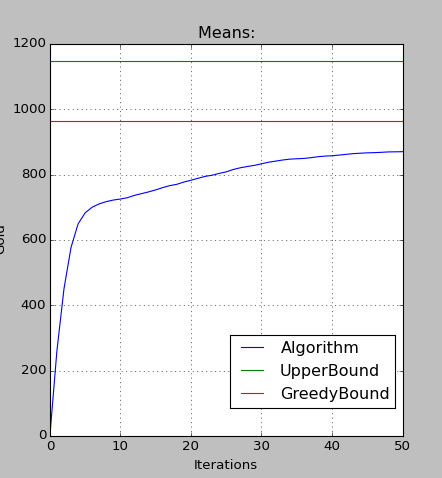
\includegraphics[width=.4\textwidth]{10ad_50r_1000it_cut.png}
  \caption{Konfiguration K1: 76\% Upper Bound, 90\% Greedy Bound}
\end{figure}
\label{fig:eval1}
\begin{figure}
  \centering
  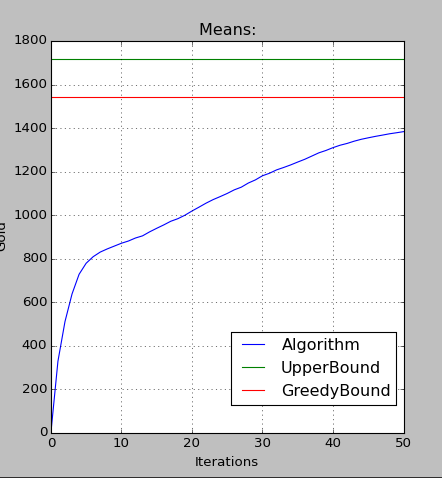
\includegraphics[width=.4\textwidth]{15ad_50r_1000it_cut.png}
  \caption{Konfiguration K2: 81\% Upper Bound, 90\% Greedy Bound}
\end{figure}
\label{fig:eval2}
\begin{figure}
  \centering
  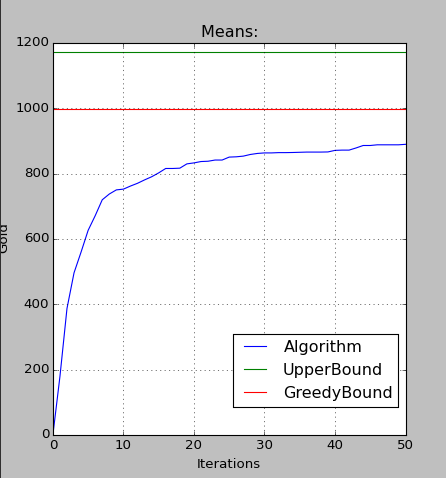
\includegraphics[width=.4\textwidth]{10ad_15ag_50r_50it_cut.png}
  \caption{Konfiguration K3: 75\% Upper Bound, 89\% Greedy Bound}
\end{figure}
\label{fig:eval3}
\begin{figure}
  \centering
  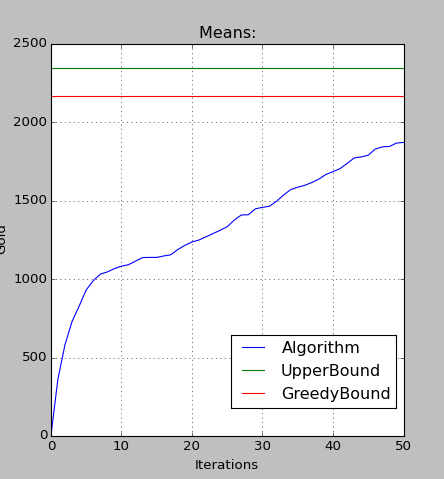
\includegraphics[width=.4\textwidth]{20ad_15ag_50r_50it_cut.png}
  \caption{Konfiguration K4: 80\% Upper Bound, 87\% Greedy Bound}
\end{figure}
\label{fig:eval4}
Insgesamt waren die Ergebnisse der Evaluation besser als erwartet, da unsere Implementierung in allen Testfällen zumindest 75\% der Upper Bound und 87\% der Greedy Bound erzielt hat. Daraus können wir schließen, dass der Gewinn in unser Implementierung im Schnitt zwischen 80 und 90\% des optimalen Gewinns liegt.
\section{Future Work}
\label{sec:Future}

Wie bereits aus der Evaluation des vorherigen Kapitels, bekannt erreicht der von uns entwickelte Algorithmus eine solide Leistung, wobei durchaus noch Verbesserungen beziehungsweise Veränderungen möglich und notwendig sind. Diese weiteren Arbeiten können und sollen sowohl die Effizienz (nähe zum Optimum) als auch die Geschwindigkeit verbessern. Es werden unter anderem Maßnahmen aufgelistete, welche den Informationsgehalt des Versuchs erhöhen, indem mehr (spezifischere) Daten betrachtet und auch berücksichtigt werden können.

\paragraph{Verteilung des Algorithmus:}
Die hier gewählte Implementierung ist kein echter verteilter Algorithmus. Die Hauptarbeit wird von einer zentralen Instanz durchgeführt, welche die Berechnungen und Entscheidungen für die Agenten (in deren Sinne) durchführt. Wenn jeder Agent als Einzelne Entität in einem verteilten Algorithmus realisiert ist, lassen sich sehr einfach individuelle Verhaltensmuster für jeweilige Abenteurer festlegen. Somit können unter anderem verschiedene Risikoaspekte mit in den Aufbau einbezogen werden. Dies bedeutet dass risikoscheue und risikoaverse Agenten aufeinander treffen können. \\
Ein weiterer Aspekt der sich zu betrachten lohnen könnte wäre, dass ein Agent A, aufgrund schlechter Erfahrungen oder Ähnlichem, unter keinen Umständen mit einem Agenten B eine Koalition bilden möchte. Hierbei könnte untersucht werden in wie weit die Effizienz des gesamten Konstruktes, durch den Ausschluss der Zusammenarbeit zweier Agenten, in Mitleidenschaft gezogen wird. In anderen Worten wie robust der Algorithmus gegenüber sich ändernden Umständen ist.

\paragraph{Optimierung der Koalitionsbildung:}
Da aktuell jeder Koalition berechnet werden muss, aufgrund des Banzhaf Power Index ist der Aufwand der Koalitionsberechnung exponentiell. Dies führt dazu, dass der Algorithmus schon bei einer vergleichsweise geringen Anzahl von Abenteurern extrem viel Zeit benötigt. Es muss demnach eine Möglichkeit gefunden werden ein im besten Fall identisches Ergebnis in geringerer Zeit zu generieren. Der intuitive Ansatz ist hierbei nicht alle Koalitionen zu betrachten, sondern eine simple Vorauswahl zu treffen welche die wichtigsten Eigenschaften bewahrt. Wie diese auszusehen hat und wie groß der Effizienzverlust ist muss ermittelt und evaluiert werden.

\paragraph{Maschinelles Lernen:} 
In der von uns entwickelten Lösung wird Maschinelles Lernen nur sehr marginal verwendet. Agenten merken sich unter anderem wie oft sie bereits an einer Koalition gescheitert sind. Wenn dieser Anteil erheblich ausgebaut werden würde und sich jede Aktion und ihr Resultat gespeichert wird, lassen sich unter Umständen ganz neue Lösungsverhalten finden, welche eher dem Optimum entsprechen. Hierbei ist allerdings nicht die Lernphase über die Dauer eines Spiels gemeint, sondern Lernen anhand von entsprechend vielen kompletten Spielen das angestrebte Ergebnis. Wahrscheinlich ließen sich mittels Lernen neue, unerwartete Lösungen mit ähnlichem beziehungsweise besserem Ergebnis finden. Dieser lernende Agent kann gegen "gewöhnliche" Agenten oder sogar Menschen spielen, diese anhand ihres Verhaltens identifizieren beziehungsweise kategorisieren und eine geeignete Strategie anwenden. Dies sei nur als Anreiz für die Einbettung maschinellen Lernens zu verstehen und erhebt nicht den Anspruch vollständig zu sein.

\paragraph{Untersuchung aller Parameter:}
Das großflächige Untersuchen sämtlicher Parameter könnte aufschlussreiche Ergebnisse liefern. In dieser Evaluation wurde nur die Menge von Agenten und Abenteuern variiert. Weitere Variationsmöglichkeiten sind:
\begin{itemize}
	\item \textit{Belohnung}: Die Verteilung von Auszahlungen der Abenteuer könnte variiert werden. Der Anstieg der Belohnung bezüglich Anforderungen könnte steiler, linear oder mittels einer beliebigen Funktion werden. Auch ein stagnierender Anstieg der Auszahlung für größere Abenteuer ist denkbar.
	\item \textit{Skillmengen}: Statt drei Skills, könnte einem Agenten eine beliebige Anzahl an Skills zugewiesen werden. Eine weitere denkbare Alternative ist, dass nicht jede Baustelle alle Skills benötigt, oder die Agenten mehr als nur einen Skill besitzen, wodurch die Verhandlung eine weitere Dimension erreicht. 
	\item \textit{Powergrößen}: Die Power jedes einzelnen Agenten, aller Agenten oder die die Abenteuer benötigen, sind weitere Variationsmöglichkeiten.
	\item \textit{Angebot}: Zum einen kann das Überangebot der Aufgaben noch verschärft oder zu ein Unterangebot abgewandelt werden. Dann würde sich auch die Frage nach dem Ergebnis verändern, da bei dieser Veränderung nicht von Interesse ist, wie viel Gold alle Agenten erwirtschaften, sondern wer grundsätzlich Gewinn bekommt und wie viel. \\
	Ein weiteres Szenario ist eine komplette Gleichverteilung. Es ist demnach möglich alle Abenteuer zu lösen ohne das ein Skillpunkt eines Abenteurers übrig bleibt. Hier stellt sich die Frage, welcher Agent wie viel vom Gewinn erwirtschaften kann.
	\item \textit{Agenten}: Die verschiedenen Verhalten die ein Agent aufweisen kann wurden bereits erläutert.
\end{itemize}




\section{Conclusion}
\label{sec:Conclusion}
Für das Zusammenführen von Agenten mit variablen Fertigkeiten und Aufgaben mit variablen Anforderungen, wird mit dem hier vorgestellten Algorithmus ein robuster und effektiver Lösungsansatz gezeigt.\\ Der Algorithmus erzielt verlässlich Lösungen nahe am theoretischen Optimum und erreicht einen Großteil des Gewinns bereits nach wenigen Iterationen. Eingeführten Variationen führten dabei nicht zu abweichenden Ergebnissen, sodass davon ausgegangen werden muss, dass Robustheit zumindest in dieser Hinsicht gegeben ist.\\ Weiterhin werden Bereiche und Eigenschaften des Algorithmus aufgezeigt, welche Potential für Anpassungen und Verbesserungen bieten.

%------------------------------------------------



%----------------------------------------------------------------------------------------
%	REFERENCE LIST
%----------------------------------------------------------------------------------------
\phantomsection
\bibliographystyle{unsrt}

%----------------------------------------------------------------------------------------

\end{document}
